\documentclass[article]{jss}\usepackage[]{graphicx}\usepackage[]{color}
% maxwidth is the original width if it is less than linewidth
% otherwise use linewidth (to make sure the graphics do not exceed the margin)
\makeatletter
\def\maxwidth{ %
  \ifdim\Gin@nat@width>\linewidth
    \linewidth
  \else
    \Gin@nat@width
  \fi
}
\makeatother

\definecolor{fgcolor}{rgb}{0.345, 0.345, 0.345}
\newcommand{\hlnum}[1]{\textcolor[rgb]{0.686,0.059,0.569}{#1}}%
\newcommand{\hlstr}[1]{\textcolor[rgb]{0.192,0.494,0.8}{#1}}%
\newcommand{\hlcom}[1]{\textcolor[rgb]{0.678,0.584,0.686}{\textit{#1}}}%
\newcommand{\hlopt}[1]{\textcolor[rgb]{0,0,0}{#1}}%
\newcommand{\hlstd}[1]{\textcolor[rgb]{0.345,0.345,0.345}{#1}}%
\newcommand{\hlkwa}[1]{\textcolor[rgb]{0.161,0.373,0.58}{\textbf{#1}}}%
\newcommand{\hlkwb}[1]{\textcolor[rgb]{0.69,0.353,0.396}{#1}}%
\newcommand{\hlkwc}[1]{\textcolor[rgb]{0.333,0.667,0.333}{#1}}%
\newcommand{\hlkwd}[1]{\textcolor[rgb]{0.737,0.353,0.396}{\textbf{#1}}}%
\let\hlipl\hlkwb

\usepackage{framed}
\makeatletter
\newenvironment{kframe}{%
 \def\at@end@of@kframe{}%
 \ifinner\ifhmode%
  \def\at@end@of@kframe{\end{minipage}}%
  \begin{minipage}{\columnwidth}%
 \fi\fi%
 \def\FrameCommand##1{\hskip\@totalleftmargin \hskip-\fboxsep
 \colorbox{shadecolor}{##1}\hskip-\fboxsep
     % There is no \\@totalrightmargin, so:
     \hskip-\linewidth \hskip-\@totalleftmargin \hskip\columnwidth}%
 \MakeFramed {\advance\hsize-\width
   \@totalleftmargin\z@ \linewidth\hsize
   \@setminipage}}%
 {\par\unskip\endMakeFramed%
 \at@end@of@kframe}
\makeatother

\definecolor{shadecolor}{rgb}{.97, .97, .97}
\definecolor{messagecolor}{rgb}{0, 0, 0}
\definecolor{warningcolor}{rgb}{1, 0, 1}
\definecolor{errorcolor}{rgb}{1, 0, 0}
\newenvironment{knitrout}{}{} % an empty environment to be redefined in TeX

\usepackage{alltt}

%% -- LaTeX packages and custom commands ---------------------------------------

%% recommended packages
\usepackage{thumbpdf,lmodern}
\usepackage{textcomp}
\usepackage[section]{placeins}
\usepackage{tabularx}
\usepackage{graphicx}
\usepackage{adjustbox}
\usepackage{makecell}
\usepackage{float}
\usepackage{longtable}
\newcommand\mc[1]{\multicolumn{1}{c}{#1}}

%% another package (only for this demo article)
\usepackage{framed}

%% new custom commands
\newcommand{\class}[1]{`\code{#1}'}
\newcommand{\fct}[1]{\code{#1()}}

%% For Sweave-based articles about R packages:
%% need no \usepackage{Sweave}
%% \SweaveOpts{engine=R, eps=FALSE, keep.source = TRUE}



%% -- Article metainformation (author, title, ...) -----------------------------

%% - \author{} with primary affiliation
%% - Separate authors by \And or \AND (in \author).
%% - \AND starts a new line, \And does not.
\author{Harry A. Smith\\Department of Biostatistics and Informatics
\\Colorado School of Public Health\\Skaggs School of Pharmacy\\and
Pharmaceutical Sciences
   \And Laura Saba\\Skaggs School of Pharmacy\\and
Pharmaceutical Sciences}
%% \Plainauthor{Achim Zeileis, Second Author}

%% - \title{} in title case
%% - \Plaintitle{} without LaTeX markup (if any)
%% - \Shorttitle{} with LaTeX markup (if any), used as running title
\title{diffEnrich: An \proglang{R} Package to Compare Functional Enrichment Between Two
Experimentally-derived Groups of Genes by Connecting to the KEGG REST API}
\Plaintitle{diffEnrich: An R Package to Compare Functional Enrichment Between Two
Experimentally-derived Groups of Genes by Connecting to the KEGG REST API}
\Shorttitle{The \proglang{R} Package diffEnrich}

%% - \Abstract{} almost as usual
\Abstract{
  \textbf{Motivation:} To aid in the biological interpretation of a list of candidate
  genes and proteins generated as part of omics studies, researchers quantitate
  the enrichment of known pathways or biological functions among the genes of
  interest. With the advent of new technologies and new experimental designs,
  it is often of interest to compare enrichment of a particular pathway between
  two gene lists (i.e., differential enrichment).
  \textbf{Results:} This package provides a number of functions that are intended to be
  used in a pipeline. Briefly, a function within the package will map
  species-specific ENTREZ gene IDs to their respective Kyoto Encyclopedia of
  Genes and Genomes (KEGG) pathways by accessing the KEGG REST API. The KEGG API
  is used to guarantee the most up-to-date pathway data from KEGG. Next, another
  function will identify significantly enriched pathways in two gene sets
  independently. The user can then identify pathways that are differentially
  enriched between the two gene sets using a third function. This package also
  provides a plotting function.
  \textbf{Availability and implementation:} diffEnrich is freely available on the
  Comprehensive R Archive Network (CRAN). Issues and bug reports can be submitted
  to the GitHub page \url{https://github.com/SabaLab/diffEnrich/issues}.
  \textbf{Supplementary information:} A step-by-step tutorial is provided on the diffEnrich
  GitHub page \url{https://github.com/SabaLab/diffEnrich}, and example data are
  included in the package.

}

%% - \Keywords{} with LaTeX markup, at least one required
%% - \Plainkeywords{} without LaTeX markup (if necessary)
%% - Should be comma-separated and in sentence case.
\Keywords{differential enrichment, KEGG REST API, \proglang{R}}
\Plainkeywords{differential enrichment, KEGG REST API, R}

%% - \Address{} of at least one author
%% - May contain multiple affiliations for each author
%%   (in extra lines, separated by \emph{and}\\).
%% - May contain multiple authors for the same affiliation
%%   (in the same first line, separated by comma).
\Address{
  Laura Saba\\
  University of Colorado\\
  Skaggs School of Pharmacy and Pharmaceutical Sciences\\
  Mail Stop C238\\
  12850 E. Montview Blvd. V20-2124\\
  Aurora, CO 80045\\
  E-mail: \email{Laura.Saba@cuanschutz.edu}
}
\IfFileExists{upquote.sty}{\usepackage{upquote}}{}
\begin{document}


%% -- Introduction -------------------------------------------------------------

%% - In principle "as usual".
%% - But should typically have some discussion of both _software_ and _methods_.
%% - Use \proglang{}, \pkg{}, and \code{} markup throughout the manuscript.
%% - If such markup is in (sub)section titles, a plain text version has to be
%%   added as well.
%% - All software mentioned should be properly \cite-d.
%% - All abbreviations should be introduced.
%% - Unless the expansions of abbreviations are proper names (like "Journal
%%   of Statistical Software" above) they should be in sentence case (like
%%   "generalized linear models" below).

\section[Introduction]{Introduction} \label{sec:intro}

Often high throughput omics studies include a functional enrichment analysis to
glean biological insight from a list of candidate genes, proteins, metabolites,
etc. Functional enrichment examines whether the number of genes in the list
associated with a biological function or particular pathway is more than would
be expected by chance. As an example, enrichment of a particular pathway among
a list of genes that are differentially expressed after an experimental
manipulation may indicate that the pathway has been altered by that
manipulation. This analysis is rather straight forward and many solutions have
been offered (e.g., \cite{HuangDW:2009}; \cite{Kuleshov:2016}; \cite{Liao:2019};
\cite{Subramanian:2005}). A wide variety of databases have also been
used to define these pathways (e.g., \cite{KEGG:2000}) and ontologies
(e.g., \cite{Ashburner:2000}).

One key component of a statistically rigorous functional enrichment analysis is
the definition of a background data set that can be used to estimate the number
of candidate genes that are ``expected'' to be associated with the pathway by
chance, e.g., if 5\% of genes in the background data set are associated with
a pathway then 5\% of candidate gene are expected to be associated with the
pathway by chance. For many study designs, the background data set is
relatively simple to define (e.g., RNA-Seq analyses where the background data
set includes genes expressed above background).

However, for some newer omics technologies, the background data set is hard to
define. For example, LC-MS analysis can be used to identify carbonylated
proteins ( \cite{Petersen:2018}; \cite{Shearn:2019}; \cite{Shearn:2018}).
With this study design, carbonylated proteins are isolated using a BH-derivation
and then LC-MS is used to identify peptides in this isolated sample. The most
appropriate background data set would be proteins present in that tissue, but
this would require a separate analytical analysis. Furthermore, most functional
enrichment analyses involve a single gene list. However, in protein modification
studies, the typical experimental design compares the presence or absence of
particular modified proteins between multiple groups.

When there are two or more gene lists to compare and the background gene list is
not clearly defined, as is often the case in protein modification experiments,
we propose a differential enrichment analysis. In this analysis, we compare the
proportion of genes/proteins from one gene list associated with a particular
pathway to the proportion of genes/proteins from a second gene list that are
associated with that pathway. To easily execute this analysis, we have designed
an R package that uses the KEGG REST API to obtain the most recent version of
the KEGG PATHWAY (\cite{KEGG:2000}) database to initially identify
functional enrichment within a gene list using the entire KEGG transcriptome as
the background data set and then to identify differentially enriched pathways
between two gene lists. This R package includes a function to generate a
``differential enrichment'' graphic.

KEGG is a database resource for understanding high-level functions of a
biological system, such as a cell, an organism and an ecosystem, from genomic
and molecular-level information \url{https://www.kegg.jp/kegg/kegg1a.html}. KEGG is
an integrated database resource consisting of eighteen databases that are
clustered into 4 main categories: 1) systems information (e.g. hierarchies
and maps), 2) genomic information (e.g. genes and proteins), 3) chemical
information (e.g. biochemical reactions), and 4) health information (e.g. human
disease and drugs) \url{https://www.kegg.jp/kegg/kegg1a.html}.


\begin{figure}[!ht]
% \centering
\begin{knitrout}
\definecolor{shadecolor}{rgb}{0.969, 0.969, 0.969}\color{fgcolor}
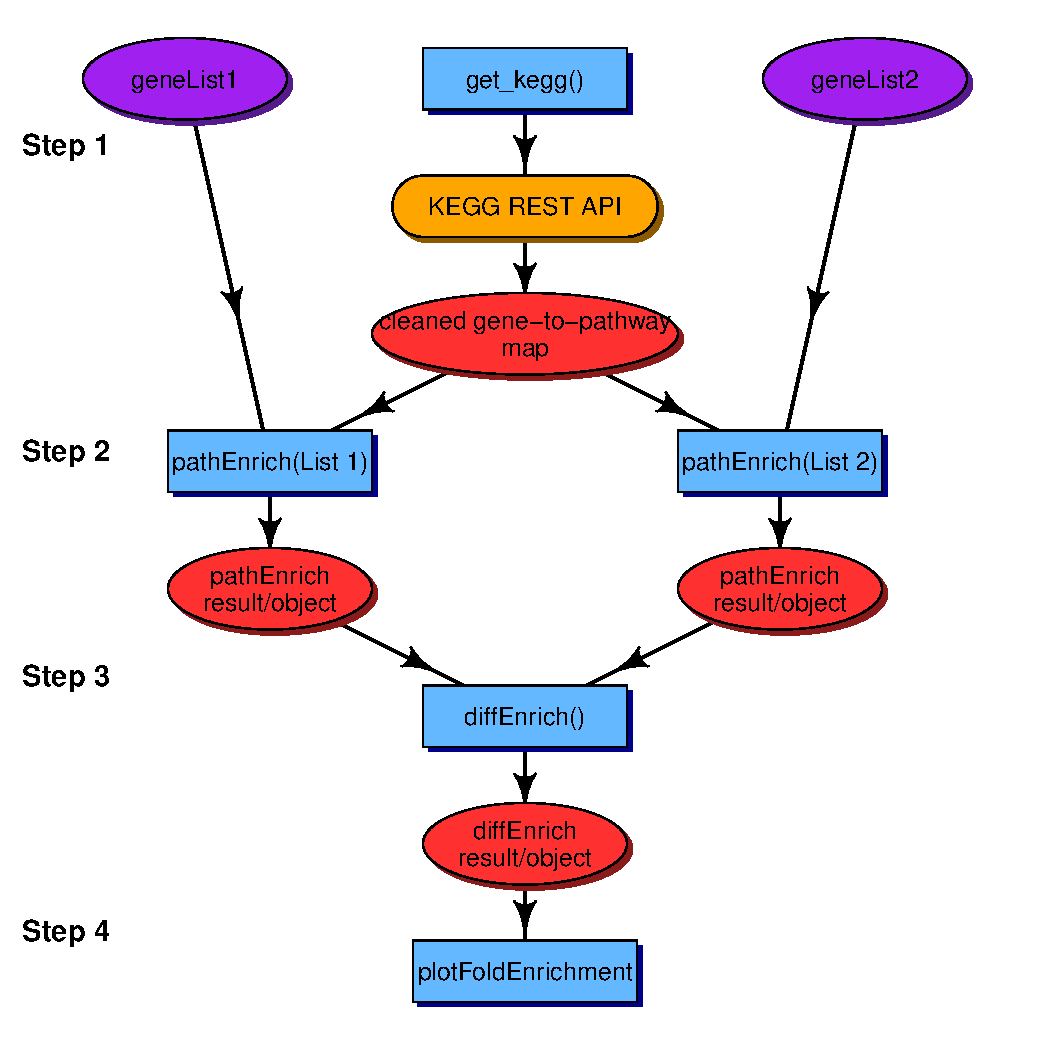
\includegraphics[width=\maxwidth]{figure/visualization-1} 

\end{knitrout}
\caption{\label{fig:flowchart} \textbf{diffEnrich Analysis pipeline.} Functions within
the diffEnrich package are represented by blue rectangles. The data that must be
provided by the user is represented by the purple ovals. Data objects generated
by a function in diffEnrich are represented by red ovals. The external call of
the \code{get\textunderscore kegg} function to the KEGG REST API is represented in yellow.}
\end{figure}

In 2012 KEGG released its first application programming interface (API), and has
been adding features and functionality ever since. There are benefits to using
an API. First, API\textquotesingle s, like KEGG\textquotesingle s, allow users to
perform customized analyses with the most up-to-date versions of the data
contained in the database. In addition, accessing the KEGG API is very easy
using statistical programming tools like R or Python and integrating data
retrieval into user\textquotesingle s code makes the
program reproducible. To further enforce reproducibilty diffEnrich adds a date
and KEGG release tag to all data files it generates from accessing the API. For
update histories and release notes for the KEGG REST API please visit
\url{https://www.kegg.jp/kegg/rest/}.

%% ------------Section 2: Features----------------------------------------------

\section[Features]{Features} \label{sec:feat}

The goal of the diffEnrich package is to compare functional enrichment between
two experimentally-derived groups of genes or proteins. This package provides
four functions that are intended to be used in an ordered pipeline
(Figure~\ref{fig:flowchart}).

\medskip

You can install the released version of diffEnrich from CRAN with:

\begin{knitrout}
\definecolor{shadecolor}{rgb}{0.969, 0.969, 0.969}\color{fgcolor}\begin{kframe}
\begin{alltt}
\hlkwd{install.packages}\hlstd{(}\hlstr{"diffEnrich"}\hlstd{)}
\end{alltt}
\end{kframe}
\end{knitrout}

\subsection{\code{get\textunderscore kegg}: Download and prepare pathways from KEGG API}

First, the \code{get\textunderscore kegg} function is used to connect to the
KEGG REST API and download the data sets required to perform downstream
analysis. Currently, this function supports three species: Homo sapiens, Mus
musculus, and Rattus norvegicus. For a given species, three data sets are
generated: 1) ncbi\textunderscore to\textunderscore kegg: this data set maps NCBI/ENTREZ gene IDs to KEGG gene
IDs, 2) kegg\textunderscore to\textunderscore pathway: this data set maps KEGG gene IDs to their respective
KEGG pathway IDs, and 3) pathway\textunderscore to\textunderscore species: this data set maps KEGG pathway IDs
to their respective pathway descriptions. This function typically completes in a
few seconds, but it is important to note that the finishing time is dependent on
the time it takes to connect to the KEGG API.

The \code{get_\textunderscore kegg} function accesses the KEGG REST API and downloads the data
sets required to perform downstream analysis. This function takes two arguments.
The first, 'species' is required. Currently, diffEnrich supports three species,
and the argument is a character string using the KEGG code: Homo sapiens
(human), use 'hsa'; Mus musculus (mouse), use 'mmu'; and Rattus norvegicus
(rat), use 'rno'. The second, 'path' is also passed as a character string, and
is the path of the directory in which the user would like to write the data sets
downloaded from the KEGG REST API. If the user does not provide a path, the data
sets will be automatically written to the current working directory using the
\code{here::here()} (\cite{kirill:2017}) functionality. These data sets will be
tab delimited files with a name describing the data, and for reproducibility,
the date they were generated and the version of KEGG when the API was accessed.
In addition to these flat files, \code{get\textunderscore kegg} will also create a named list
in R with the three relevant KEGG data sets. The names of this list will
describe the data set, and are described in Table 1.

\begin{knitrout}
\definecolor{shadecolor}{rgb}{0.969, 0.969, 0.969}\color{fgcolor}\begin{kframe}
\begin{alltt}
\hlcom{## Load package}
\hlkwd{suppressMessages}\hlstd{(}\hlkwd{library}\hlstd{(diffEnrich))}
\hlcom{## run get_kegg() using rat}
\hlstd{kegg_rno} \hlkwb{<-} \hlkwd{get_kegg}\hlstd{(}\hlstr{'rno'}\hlstd{)}
\end{alltt}


{\ttfamily\noindent\itshape\color{messagecolor}{\#\# 3 data sets will be written as tab delimited text files}}

{\ttfamily\noindent\itshape\color{messagecolor}{\#\# File location: /Users/harry/Documents/Saba\_Lab/diffEnrich}}

{\ttfamily\noindent\itshape\color{messagecolor}{\#\# Kegg Release: Release\_92.0+\_12-05\_Dec\_19}}\end{kframe}
\end{knitrout}

\textbf{Note:} Because it is assumed that a user might want to use the data sets
generated by \code{get\textunderscore kegg}, it is careful not to overwrite data
sets with exact names. \code{get\textunderscore kegg} checks the path provided
for data sets generated 'same-day/same-version', and if it finds even one of the
three, it will not re-write any of the data sets. It will still however, let the
user know it is not writing out new data sets and still generate the named list
object. Users can generate 'same-day/same-version' data sets in different
directories if they so choose.

\begin{knitrout}
\definecolor{shadecolor}{rgb}{0.969, 0.969, 0.969}\color{fgcolor}\begin{kframe}
\begin{alltt}
\hlcom{## run get_kegg() using rat}
\hlstd{kegg_rno} \hlkwb{<-} \hlkwd{get_kegg}\hlstd{(}\hlstr{'rno'}\hlstd{)}
\end{alltt}


{\ttfamily\noindent\itshape\color{messagecolor}{\#\# These files already exist in your working directory. New files will not be generated.}}

{\ttfamily\noindent\itshape\color{messagecolor}{\#\# Kegg Release: Release\_92.0+\_12-05\_Dec\_19}}\end{kframe}
\end{knitrout}

Additionally, \code{get\textunderscore kegg} can be used to read in saved
versions of the txt files generated from a previous call, and generate an R list
object that is compatible with downstream functions.

\begin{knitrout}
\definecolor{shadecolor}{rgb}{0.969, 0.969, 0.969}\color{fgcolor}\begin{kframe}
\begin{alltt}
\hlcom{## run get_kegg() using rat}
\hlstd{date} \hlkwb{<-} \hlkwd{as.character}\hlstd{(}\hlkwd{Sys.Date}\hlstd{())}
\hlstd{kegg_rno} \hlkwb{<-} \hlkwd{get_kegg}\hlstd{(}\hlkwc{read} \hlstd{=} \hlnum{TRUE}\hlstd{,}
                     \hlkwc{path} \hlstd{= here}\hlopt{::}\hlkwd{here}\hlstd{(),}
                     \hlkwc{date} \hlstd{= date,}
                     \hlkwc{release} \hlstd{=} \hlstr{"92"}\hlstd{)}
\end{alltt}


{\ttfamily\noindent\itshape\color{messagecolor}{\#\# Reading in the following files:}}

{\ttfamily\noindent\itshape\color{messagecolor}{\#\# ncbi\_to\_kegg2019-12-05Release\_92.0+\_12-05\_Dec\_19.txt}}

{\ttfamily\noindent\itshape\color{messagecolor}{\#\# kegg\_to\_pathway2019-12-05Release\_92.0+\_12-05\_Dec\_19.txt}}

{\ttfamily\noindent\itshape\color{messagecolor}{\#\# pathway\_to\_species2019-12-05Release\_92.0+\_12-05\_Dec\_19.txt}}

{\ttfamily\noindent\itshape\color{messagecolor}{\#\# File location: /Users/harry/Documents/Saba\_Lab/diffEnrich}}\end{kframe}
\end{knitrout}

\begin{table}[ht!]
  \centering
  \caption{\label{tab:description} Description of the data sets retrieved by \code{get\textunderscore kegg}'s
connection to the KEGG REST API.}
  \begin{adjustbox}{width=\textwidth}
  \begin{tabular}{rr}
\hline
\code{get\textunderscore kegg} list object & Description \\ \hline
ncbi\textunderscore to\textunderscore kegg                & ncbi gene ID <-- mapped to --> KEGG gene ID \\
kegg\textunderscore to\textunderscore pathway             & KEGG gene ID <-- mapped to --> KEGG pathway ID \\
pathway\textunderscore to\textunderscore species          & KEGG pathway ID <-- mapped to --> KEGG pathway species description \\ \hline
\end{tabular}
\end{adjustbox}
\end{table}

\subsection{\code{pathEnrich}: Perform enrichment analysis of individual gene sets.}

In this step, the \code{pathEnrich} function is used to identify KEGG pathways
that are enriched (i.e. over-represented) based on a gene list of interest
provided by the user. User gene lists must be ENTREZ gene IDs. If a user only
has gene symbols, the \code{clusterProfiler} package (3.9) (Yu:2012) offers a
function (\code{bitr}) that maps gene symbols and Ensembl IDs to ENTREZ gene
IDs. An example of this function's use can be found in their vignette
(\url{https://yulab-smu.github.io/clusterProfiler-book/chapter14.html#bitr}).

\begin{knitrout}
\definecolor{shadecolor}{rgb}{0.969, 0.969, 0.969}\color{fgcolor}\begin{kframe}
\begin{alltt}
\hlcom{## View sample gene lists from package data}
\hlkwd{head}\hlstd{(geneLists}\hlopt{$}\hlstd{list1)}
\end{alltt}
\begin{verbatim}
## [1] "361692"    "293654"    "293655"    "500974"    "100361529"
## [6] "171434"
\end{verbatim}
\begin{alltt}
\hlkwd{head}\hlstd{(geneLists}\hlopt{$}\hlstd{list2)}
\end{alltt}
\begin{verbatim}
## [1] "315547" "315548" "315549" "315550" "50938"  "58856"
\end{verbatim}
\end{kframe}
\end{knitrout}

The pathEnrich function will only use the genes from the list provided that are
also in the KEGG database. The \code{pathEnrich} function should be run at least
twice, once for the genes of interest in list 1 and once for the genes of
interest in list 2. Each \code{pathEnrich} call generates a data frame
summarizing the results of enrichment analyses in which a Fisher’s Exact test is
used to identify which KEGG pathways are enriched within the user’s list of
genes compared to all genes annotated to a KEGG pathway. Users can limit which
pathways are tested by requiring that they contain a minimum number of genes
from the list, and this can be set by changing the 'N' arguement. The default is
that a KEGG pathway must contain at least 2 genes (N = 2) from the user’s list
to be tested.



By default, p-values from the Fisher’s Exact test are adjusted for multiple
comparisons with a False Discovery Rate (FDR) (Benjamini:1995), however users
have the option of choosing any type of multiple testing correction supported
by \code{p.adjust}. In addition to the unadjusted p-value and FDR, pathEnrich
will calculate for each KEGG pathway, its fold enrichment defined as the ratio
of number of genes observed from the gene list annotated to the KEGG pathway to
the expected number of genes from the gene list to be annotated to the KEGG
pathway by chance. An example of the first 6 results generated by \code{pathEnrich}
are in displayed below. For a detailed description of the variables in this table see Table 2.

\begin{knitrout}
\definecolor{shadecolor}{rgb}{0.969, 0.969, 0.969}\color{fgcolor}\begin{kframe}
\begin{alltt}
\hlkwd{head}\hlstd{(list1_pe}\hlopt{$}\hlstd{enrich_table)}
\end{alltt}
\begin{verbatim}
##     KEGG_PATHWAY_ID
## 95         rno04530
## 172        rno05135
## 194        rno05210
## 212        rno05231
## 197        rno05213
## 66         rno04144
##                                   KEGG_PATHWAY_description
## 95                Tight junction - Rattus norvegicus (rat)
## 172           Yersinia infection - Rattus norvegicus (rat)
## 194            Colorectal cancer - Rattus norvegicus (rat)
## 212 Choline metabolism in cancer - Rattus norvegicus (rat)
## 197           Endometrial cancer - Rattus norvegicus (rat)
## 66                   Endocytosis - Rattus norvegicus (rat)
##     KEGG_PATHWAY_cnt KEGG_PATHWAY_in_list KEGG_DATABASE_cnt
## 95               170                   19              8856
## 172              128                   16              8856
## 194               88                   12              8856
## 212               99                   12              8856
## 197               58                    9              8856
## 66               275                   22              8856
##     KEG_DATABASE_in_list expected     enrich_p        p_adj
## 95                   295 5.662827 3.485551e-06 0.0005387284
## 172                  295 4.263776 4.919894e-06 0.0005387284
## 194                  295 2.931346 3.179635e-05 0.0023211334
## 212                  295 3.297764 1.032192e-04 0.0044701134
## 197                  295 1.932023 1.132216e-04 0.0044701134
## 66                   295 9.160456 1.224689e-04 0.0044701134
##     fold_enrichment
## 95         3.355214
## 172        3.752542
## 194        4.093683
## 212        3.638829
## 197        4.658328
## 66         2.401627
\end{verbatim}
\end{kframe}
\end{knitrout}




%\begin{table}[hp!]
%\centering
\begin{longtable}{cc}
  \caption{Description of columns in dataframe generated by pathEnrich.}
  % \begin{adjustbox}{width=\textwidth}
  % \begin{tabular}{rll}
  \hline
Column Names & Column Description \\
  \hline
  \endhead
  \hline
  \endfoot
KEGG\_PATHWAY\_ID & \makecell{KEGG Pathway Identifier \\} \\
& & \\
KEGG\_PATHWAY\_description & \makecell{Description of KEGG Pathway \\ (provided by KEGG) \\ } \\
  & & \\
KEGG\_PATHWAY\_cnt & \makecell{Number of Genes in KEGG Pathway} \\
& & \\
KEGG\_PATHWAY\_in\_list & \makecell{Number of Genes from  \\ gene list in KEGG Pathway} \\
& & \\
KEGG\_DATABASE\_cnt & \makecell{Number of Genes in KEGG Database} \\
& & \\
KEGG\_DATABASE\_in\_list & \makecell{Number of Genes from \\ gene list in KEGG Database} \\
& & \\
expected & \makecell{Expected number of genes \\ from list to be in \\ KEGG pathway by chance} \\
& & \\
enrich\_p & \makecell{P-value for enrichment within \\ the KEGG pathway for list genes} \\
& & \\
p\_adj & \makecell{Multiple testing adjusted enrichment \\ p-values (default = False Discovery Rate \\ (Benjamini and Hochberg, 1995))} \\
& & \\
fold\_enrichment & \makecell{Ratio of number of genes observed  \\ from the gene list annotated to the \\ KEGG pathway to the number of genes  \\ expected from the gene list to  \\ be annotated to the KEGG pathway if  \\ there was no enrichment \\ (i.e. KEGG\_PATHWAY\_in\_list/expected)} \\
  % \end{tabular}
% \end{adjustbox}
\end{longtable}
%\end{table}


S3 generic functions for \code{print} and \code{summary} are provided.
The \code{print} function prints the results table as a \code{tibble}, and the
\code{summary} function returns the number of pathways that reached statistical
significance as well as their descriptions, the number of genes used from the
KEGG data base, the KEGG species, and the method used for multiple testing
correction.

\begin{knitrout}
\definecolor{shadecolor}{rgb}{0.969, 0.969, 0.969}\color{fgcolor}\begin{kframe}
\begin{alltt}
\hlkwd{summary}\hlstd{(list1_pe)}
\end{alltt}
\begin{verbatim}
## 219 KEGG pathways were tested. 
##  Only KEGG pathways that contained at least 2 genes from gene_list were tested. 
##  KEGG pathway species: Rattus norvegicus (rat)
##  8856 genes from gene_list were in the KEGG data pull. 
##  p-value adjustment method: BH
##  36 pathways reached statistical significance after multiple testing correction at a cutoff of 0.05. 
##  
## Significant pathways: 
##  Tight junction
## Yersinia infection
## Colorectal cancer
## Choline metabolism in cancer
## Endometrial cancer
## Endocytosis
## Neurotrophin signaling pathway
## Thermogenesis
## Oocyte meiosis
## VEGF signaling pathway
## Thyroid hormone signaling pathway
## Hippo signaling pathway
## T cell receptor signaling pathway
## Apoptosis
## Hepatocellular carcinoma
## MAPK signaling pathway
## Focal adhesion
## Salmonella infection
## Non-alcoholic fatty liver disease (NAFLD)
## ErbB signaling pathway
## Sphingolipid signaling pathway
## Pancreatic cancer
## Progesterone-mediated oocyte maturation
## Alzheimer disease
## Endocrine resistance
## Adrenergic signaling in cardiomyocytes
## IL-17 signaling pathway
## Chronic myeloid leukemia
## Dopaminergic synapse
## Prostate cancer
## EGFR tyrosine kinase inhibitor resistance
## Hepatitis C
## Ras signaling pathway
## Acute myeloid leukemia
## Insulin signaling pathway
## Fc epsilon RI signaling pathway
\end{verbatim}
\end{kframe}
\end{knitrout}

\subsection{\code{diffEnrich}: Identify differentially enriched KEGG pathways.}

The \code{diffEnrich} function merges results from the \code{pathEnrich} function
generated in section 2.2. This merged data set is then used to perform differential
enrichment using a Fisher’s exact test as described in 2.2. The resulting odds
ratio is defined as the odds of a gene from list 2 belonging to a given KEGG
pathway divided by the odds of a gene from list 1 belonging to a given KEGG
pathway. Users have the same options for multiple testing methods that are
provided in the \code{pathEnrich} function. KEGG pathways that do not contain
any genes from either gene list (e.g. ‘rno04530’ contains 0 genes from list 1
and 0 genes from list 2) are removed from the analysis. If this is the case a
warning will be printed that tells the user how many pathways were removed.
This can be avoided by setting the 'N' parameter to a value > 0 in the
\code{pathEnrich calls}. This diffEnrich function generates a table that
contains the results from the analyses performed in section 2.2 for each gene
list as well as odds ratios and their associated unadjusted and adjusted
p-values for each KEGG pathway. For a detailed description of the results
generated by \code{diffEnrich} see Table 3, and an example of the first 6
results generated by \code{diffEnrich} are displayed below.

\begin{knitrout}
\definecolor{shadecolor}{rgb}{0.969, 0.969, 0.969}\color{fgcolor}\begin{kframe}
\begin{alltt}
\hlcom{## Perform differential enrichment}
\hlstd{diff_enrich} \hlkwb{<-} \hlkwd{diffEnrich}\hlstd{(}\hlkwc{list1_pe} \hlstd{= list1_pe,}
                          \hlkwc{list2_pe} \hlstd{= list2_pe,}
                          \hlkwc{method} \hlstd{=} \hlstr{'none'}\hlstd{,}
                          \hlkwc{cutoff} \hlstd{=} \hlnum{0.05}\hlstd{)}
\end{alltt}
\end{kframe}
\end{knitrout}

\begin{knitrout}
\definecolor{shadecolor}{rgb}{0.969, 0.969, 0.969}\color{fgcolor}\begin{kframe}
\begin{alltt}
\hlkwd{head}\hlstd{(diff_enrich}\hlopt{$}\hlstd{de_table)}
\end{alltt}
\begin{verbatim}
##          KEGG_PATHWAY_ID
## rno04530        rno04530
## rno05135        rno05135
## rno05210        rno05210
## rno05213        rno05213
## rno04660        rno04660
## rno04657        rno04657
##                                             KEGG_PATHWAY_description
## rno04530                    Tight junction - Rattus norvegicus (rat)
## rno05135                Yersinia infection - Rattus norvegicus (rat)
## rno05210                 Colorectal cancer - Rattus norvegicus (rat)
## rno05213                Endometrial cancer - Rattus norvegicus (rat)
## rno04660 T cell receptor signaling pathway - Rattus norvegicus (rat)
## rno04657           IL-17 signaling pathway - Rattus norvegicus (rat)
##          KEGG_PATHWAY_cnt KEGG_DATABASE_cnt KEGG_PATHWAY_in_list1
## rno04530              170              8856                    19
## rno05135              128              8856                    16
## rno05210               88              8856                    12
## rno05213               58              8856                     9
## rno04660              106              8856                    11
## rno04657               95              8856                     9
##          KEGG_DATABASE_in_list1 expected_list1 enrich_p_list1
## rno04530                    295       5.662827   3.485551e-06
## rno05135                    295       4.263776   4.919894e-06
## rno05210                    295       2.931346   3.179635e-05
## rno05213                    295       1.932023   1.132216e-04
## rno04660                    295       3.530939   7.743416e-04
## rno04657                    295       3.164521   4.270915e-03
##           p_adj_list1 fold_enrichment_list1 KEGG_PATHWAY_in_list2
## rno04530 0.0005387284              3.355214                   131
## rno05135 0.0005387284              3.752542                   105
## rno05210 0.0023211334              4.093683                    81
## rno05213 0.0044701134              4.658328                    55
## rno04660 0.0129121321              3.115318                    79
## rno04657 0.0346418644              2.844032                    59
##          KEGG_DATABASE_in_list2 expected_list2 enrich_p_list2
## rno04530                   5308      101.89250   1.459992e-06
## rno05135                   5308       76.71906   5.537739e-08
## rno05210                   5308       52.74435   9.806872e-12
## rno05213                   5308       34.76332   1.160182e-09
## rno04660                   5308       63.53297   1.107477e-03
## rno04657                   5308       56.93993   3.737223e-01
##           p_adj_list2 fold_enrichment_list2 odd_ratio diff_enrich_p
## rno04530 5.568342e-06              1.285669 0.3676651  0.0002935876
## rno05135 2.594826e-07              1.368630 0.3520039  0.0005434729
## rno05210 1.237175e-10              1.535709 0.3655602  0.0032572306
## rno05213 8.849757e-09              1.582127 0.3328275  0.0058774642
## rno04660 2.256227e-03              1.243449 0.3901694  0.0072047984
## rno04657 4.591045e-01              1.036180 0.3572935  0.0087537607
##          diff_enrich_adjusted
## rno04530         0.0002935876
## rno05135         0.0005434729
## rno05210         0.0032572306
## rno05213         0.0058774642
## rno04660         0.0072047984
## rno04657         0.0087537607
\end{verbatim}
\end{kframe}
\end{knitrout}

The result of the \code{diffEnrich} call is a list object that
contains a data frame with the estimated odds ratio generated
by the Fisher's Exact test and the associated p-value. S3 generic
functions for \code{print} and \code{summary} are provided. The
\code{print} function prints the results table as a \code{tibble},
and the \code{summary} function returns the number of pathways
that reached statistical significance as well as their descriptions,
the number of genes used from the KEGG database, the KEGG species,
the number of pathways that were shared (i.e. had at least N gene
from each gene list present in the pathway based on what the user
chose for N in \code{pathEnrich}) between the gene lists and the
method used for multiple testing correction.



%\begin{table}[ht]
%\centering
%\begin{tabular}{rll}
\begin{longtable}{cc}
  \caption{Description of columns in dataframe generated by diffEnrich}
  \hline
 & Column Names & Column Description \\
  \hline
  \endhead
  \hline
  \endfoot
KEGG\_PATHWAY\_ID & \makecell{KEGG Pathway Identifier} \\
& & \\
KEGG\_PATHWAY\_description & \makecell{Description of KEGG Pathway \\ (provided by KEGG)} \\
& & \\
KEGG\_PATHWAY\_cnt & \makecell{Number of Genes in KEGG Pathway} \\
& & \\
KEGG\_DATABASE\_cnt & \makecell{Number of Genes in KEGG Database} \\
& & \\
KEGG\_PATHWAY\_in\_list1 & \makecell{Number of Genes from  \\ gene list 1 in KEGG Pathway} \\
& & \\
KEGG\_DATABASE\_in\_list1 & \makecell{Number of Genes from \\ gene list 1 in KEGG Database} \\
& & \\
expected\_list1 & \makecell{Expected number of genes \\ from list 1 to be in \\ KEGG pathway by chance} \\
& & \\
enrich\_p\_list1 & \makecell{P-value for enrichment of \\ list 1 genes related to \\ KEGG pathway} \\
& & \\
p\_adj\_list1 & \makecell{Multiple testing adjusted enrichment \\ p-values from gene list 1 \\ (default = False Discovery Rate \\ (Benjamini and Hochberg, 1995))} \\
& & \\
fold\_enrichment\_list1 & \makecell{Ratio of number of genes \\ observed from gene list 1 \\ annotated to the KEGG pathway \\ to the number of genes expected \\ from gene list 1 annotated to \\ the KEGG pathway if there was no \\ enrichment (i.e. KEGG\_PATHWAY\_in\_list1/expected\_list1)} \\
& & \\
KEGG\_PATHWAY\_in\_list2 & \makecell{Number of Genes from gene \\ list 2 in KEGG Pathway} \\
& & \\
KEGG\_DATABASE\_in\_list2 & \makecell{Number of Genes from gene \\ list 2 in KEGG Database} \\
& & \\
expected\_list2 & \makecell{Expected number of genes \\ from list 2 to be in \\ KEGG pathway by chance} \\
& & \\
enrich\_p\_list2 & \makecell{P-value for enrichment of \\ list 2 genes related to \\ KEGG pathway} \\
& & \\
p\_adj\_list2 & \makecell{Multiple testing adjusted enrichment \\ p-values from gene list 2 \\ (default = False Discovery Rate \\ (Benjamini and Hochberg, 1995))} \\
& & \\
fold\_enrichment\_list2 & \makecell{Ratio of number of genes observed \\ from gene list 2 \\ annotated to the KEGG pathway \\ to the number of genes expected \\ from gene list 2 annotated to \\ the KEGG pathway if there was no \\ enrichment (i.e. KEGG\_PATHWAY\_in\_list2/expected\_list2)} \\
& & \\
odd\_ratio & \makecell{Odds of a gene from list 2 being \\ from this KEGG pathway / Odds of a gene from list 1\\  being from this KEGG pathway} \\
& & \\
diff\_enrich\_p & \makecell{P-value for differential enrichment \\ of this KEGG pathway between \\ list 1 and list 2} \\
& & \\
diff\_enrich\_adjusted & \makecell{Multiple testing adjusted differential \\ enrichment p-values \\ (default = False Discovery Rate \\ (Benjamini and Hochberg, 1995))} \\
   \hline
%\end{tabular}
\end{longtable}

\begin{knitrout}
\definecolor{shadecolor}{rgb}{0.969, 0.969, 0.969}\color{fgcolor}\begin{kframe}
\begin{alltt}
\hlkwd{summary}\hlstd{(diff_enrich)}
\end{alltt}
\begin{verbatim}
## 219 KEGG pathways were shared between gene lists and were tested. 
##  KEGG pathway species: Rattus norvegicus (rat)
##  8856 genes from gene_list were in the KEGG data pull. 
##  p-value adjustment method: none
##  19 pathways reached statistical significance after multiple testing correction at a cutoff of 0.05. 
##  
## Significant pathways: 
##  Tight junction
## Yersinia infection
## Colorectal cancer
## Endometrial cancer
## T cell receptor signaling pathway
## IL-17 signaling pathway
## Salmonella infection
## Choline metabolism in cancer
## Endocytosis
## VEGF signaling pathway
## Oocyte meiosis
## Thermogenesis
## Hippo signaling pathway
## Neurotrophin signaling pathway
## Apoptosis
## Hepatocellular carcinoma
## Fc epsilon RI signaling pathway
## Thyroid hormone signaling pathway
## Alzheimer disease
\end{verbatim}
\end{kframe}
\end{knitrout}

\subsection{\code{plotFoldEnrichment}}

\code{plotFoldEnrichment} generates a grouped bar plot using
\code{ggplot2} (\cite{Hadley:2106}) and the \code{ggnewscale}
package (\cite{Elio:2019}). There are 3 arguments: 1)
\code{de_res} is the dataframe generated from the
\code{diffEnrich} function, 2) \code{pval} is the threshold
for the adjusted p-value associated with differential
enrichment that will filter which KEGG pathways to plot, and
3) after filtering based on \code{pval}, \code{N} tells the
function how many pathways to plot. It is important to make
a note that the significance of the fold change is associated
with the number of genes in the gene list. Notice that in this
example the pathways in gene list 2 have smaller fold changes
(shorter bars) than those in list 1, but that many of them are
more significant (darker blue). This is because there are
more genes in gene list 2 compared to gene list 1.

\begin{figure}[H]
% \centering
\begin{knitrout}
\definecolor{shadecolor}{rgb}{0.969, 0.969, 0.969}\color{fgcolor}\begin{kframe}
\begin{alltt}
\hlcom{## Plot fold enrichment}
\hlkwd{plotFoldEnrichment}\hlstd{(}\hlkwc{de_res} \hlstd{= diff_enrich,} \hlkwc{pval} \hlstd{=} \hlnum{0.05}\hlstd{,} \hlkwc{N} \hlstd{=} \hlnum{5}\hlstd{)}
\end{alltt}
\end{kframe}
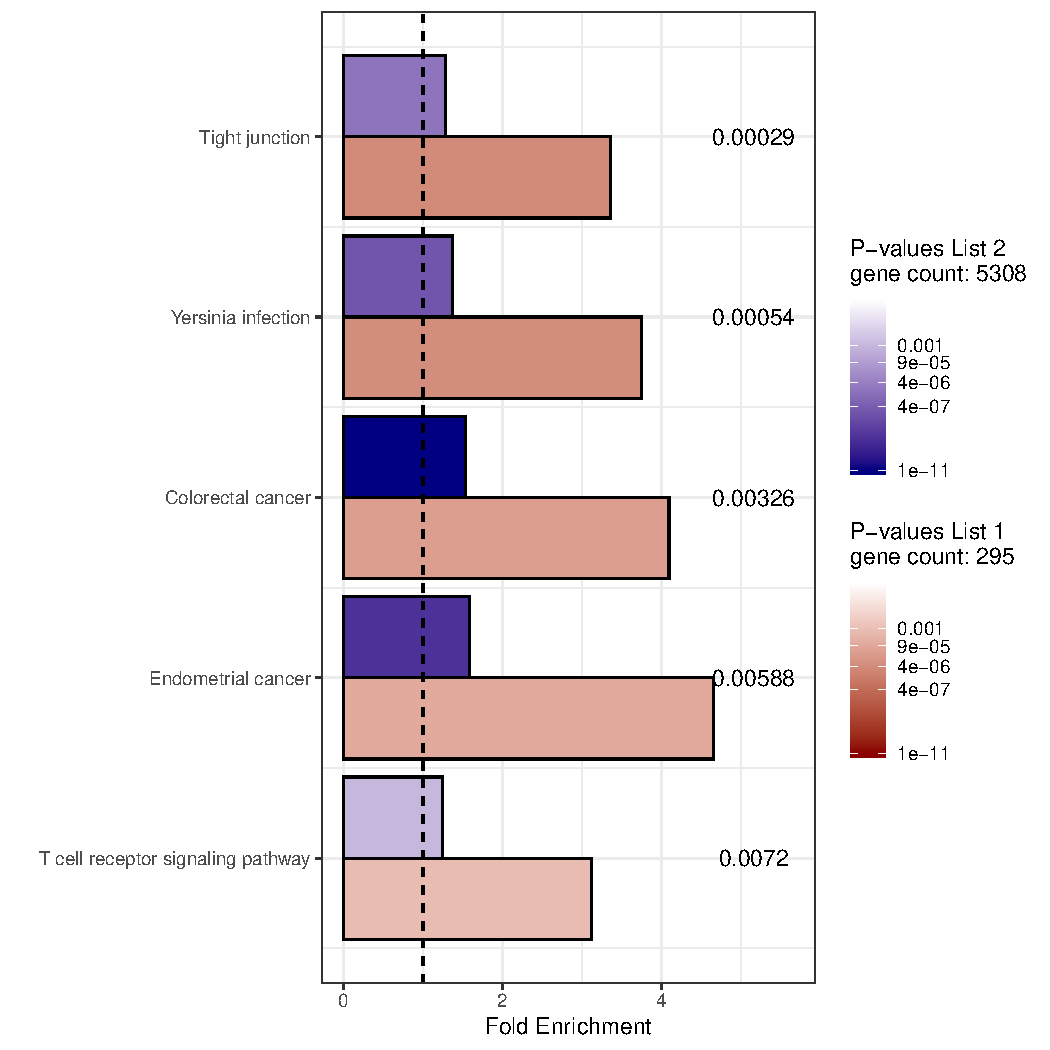
\includegraphics[width=5.0in,height=4in]{figure/visualization_2-1} 

\end{knitrout}
\caption{\label{fig:barchart} \textbf{Example of a differential enrichment graphic.}
KEGG pathways are plotted on the y-axis and fold enrichment is
plotted on the x-axis. Each KEGG pathway has a bar depicting its
fold enrichment in list 1 (red) and its fold enrichment in list 2
(blue). The transparency of the bars correspond to the unadjusted
p-value for the pathway's enrichment in the given list. The p-value
presented as text to the right of each pair of bars is the adjusted
p-value (user defined: default is FDR) associated with the
differential enrichment of the pathway between the two lists, and
the pathways are ordered from top to bottom by this p-value (i.e.
smallest p-value on top of plot, and largest p-value on bottom of
plot). The dotted line represents no enrichment (i.e a fold enrichment of 1).
The number of genes used for analysis from each gene list (recall
that this number may not be the same as the number of genes in
the user’s original list) are reported below their respective
p-values in the legend. In this example, all five pathways are
differentially enriched with more enrichment in List 1 than in
List 2.}
\end{figure}

%% -----Supplementary Information------------------------------------
% \section[Supplementary Information]{Supplementary Information} \label{sec:supinfo}



% \begin{table}[H]
%   \centering
%   \caption{Supplementary Table 1. First 6 results generated by pathEnrich.}
%   \begin{adjustbox}{width=\textwidth, angle=90}
%   \fontsize{90}{125}\selectfont
%   \begin{tabular}{rllrrrrrrrr}
%   \hline
%  & KEGG\_PATHWAY\_ID & KEGG\_PATHWAY\_description & KEGG\_PATHWAY\_cnt & KEGG\_PATHWAY\_in\_list & KEGG\_DATABASE\_cnt & KEG\_DATABASE\_in\_list & expected & enrich\_p & p\_adj & fold\_enrichment \\
%   \hline
% 95 & rno04530 & Tight junction - Rattus norvegicus (rat) & 170 & 19.00 & 8856 & 295 & 5.66 & 0.00 & 0.00 & 3.36 \\
%   172 & rno05135 & Yersinia infection - Rattus norvegicus (rat) & 128 & 16.00 & 8856 & 295 & 4.26 & 0.00 & 0.00 & 3.75 \\
%   194 & rno05210 & Colorectal cancer - Rattus norvegicus (rat) &  88 & 12.00 & 8856 & 295 & 2.93 & 0.00 & 0.00 & 4.09 \\
%   212 & rno05231 & Choline metabolism in cancer - Rattus norvegicus (rat) &  99 & 12.00 & 8856 & 295 & 3.30 & 0.00 & 0.00 & 3.64 \\
%   197 & rno05213 & Endometrial cancer - Rattus norvegicus (rat) &  58 & 9.00 & 8856 & 295 & 1.93 & 0.00 & 0.00 & 4.66 \\
%   66 & rno04144 & Endocytosis - Rattus norvegicus (rat) & 275 & 22.00 & 8856 & 295 & 9.16 & 0.00 & 0.00 & 2.40 \\
%    \hline
%   \end{tabular}
% \end{adjustbox}
% \end{table}



% \begin{table}[H]
% \centering
%   \caption{Supplementary Table 2. First 6 results generated by diffEnrich}
%   \begin{adjustbox}{width=\textwidth, angle=90}
%   \fontsize{50}{80}\selectfont
% \begin{tabular}{rllrrrrrrrrrrrrrrrrr}
%   \hline
%  & KEGG\_PATHWAY\_ID & KEGG\_PATHWAY\_description & KEGG\_PATHWAY\_cnt & KEGG\_DATABASE\_cnt & KEGG\_PATHWAY\_in\_list1 & KEGG\_DATABASE\_in\_list1 & expected\_list1 & enrich\_p\_list1 & p\_adj\_list1 & fold\_enrichment\_list1 & KEGG\_PATHWAY\_in\_list2 & KEGG\_DATABASE\_in\_list2 & expected\_list2 & enrich\_p\_list2 & p\_adj\_list2 & fold\_enrichment\_list2 & odd\_ratio & diff\_enrich\_p & diff\_enrich\_adjusted \\
%   \hline
% rno04530 & rno04530 & Tight junction - Rattus norvegicus (rat) & 170 & 8856 & 19.00 & 295 & 5.66 & 0.00 & 0.00 & 3.36 & 131.00 & 5308 & 101.89 & 0.00 & 0.00 & 1.29 & 0.37 & 0.00 & 0.00 \\
%   rno05135 & rno05135 & Yersinia infection - Rattus norvegicus (rat) & 128 & 8856 & 16.00 & 295 & 4.26 & 0.00 & 0.00 & 3.75 & 105.00 & 5308 & 76.72 & 0.00 & 0.00 & 1.37 & 0.35 & 0.00 & 0.00 \\
%   rno05210 & rno05210 & Colorectal cancer - Rattus norvegicus (rat) &  88 & 8856 & 12.00 & 295 & 2.93 & 0.00 & 0.00 & 4.09 & 81.00 & 5308 & 52.74 & 0.00 & 0.00 & 1.54 & 0.37 & 0.00 & 0.00 \\
%   rno05213 & rno05213 & Endometrial cancer - Rattus norvegicus (rat) &  58 & 8856 & 9.00 & 295 & 1.93 & 0.00 & 0.00 & 4.66 & 55.00 & 5308 & 34.76 & 0.00 & 0.00 & 1.58 & 0.33 & 0.01 & 0.01 \\
%   rno04660 & rno04660 & T cell receptor signaling pathway - Rattus norvegicus (rat) & 106 & 8856 & 11.00 & 295 & 3.53 & 0.00 & 0.01 & 3.12 & 79.00 & 5308 & 63.53 & 0.00 & 0.00 & 1.24 & 0.39 & 0.01 & 0.01 \\
%   rno04657 & rno04657 & IL-17 signaling pathway - Rattus norvegicus (rat) &  95 & 8856 & 9.00 & 295 & 3.16 & 0.00 & 0.03 & 2.84 & 59.00 & 5308 & 56.94 & 0.37 & 0.46 & 1.04 & 0.36 & 0.01 & 0.01 \\
%    \hline
% \end{tabular}
% \end{adjustbox}
% \end{table}


%% ----------------------------------------------------------------------
\bibliography{refs}





%% ----------------------------------------------------------------------


\end{document}
